\subsection{Phénomène}

\begin{definition}
Le \tdef{phénomène de diffraction} est le comportement des \abr{ops} en présence d'obstacles.
\end{definition}



\subsection{Diffraction à travers une fente}

\begin{propriete}[admis]
Lorsqu'une \abr{ops} plane de longueur d'onde $\lambda$ traverse une fente de largeur $a$ \imp{perpendiculaire à son sens de propagation}, elle ressort en divergeant. L'amplitude diffractée est importante dans un secteur dont le sommet est le centre de la fente et de demi-ouverture angulaire $\theta$ tel que :
\[\sin \theta \simeq \frac{\lambda}{a}\]

\begin{figure}[H]
\begin{center}
\begin{tikzpicture}[thick]
\node[anchor=north west, inner sep=0] (image) at (0,0) {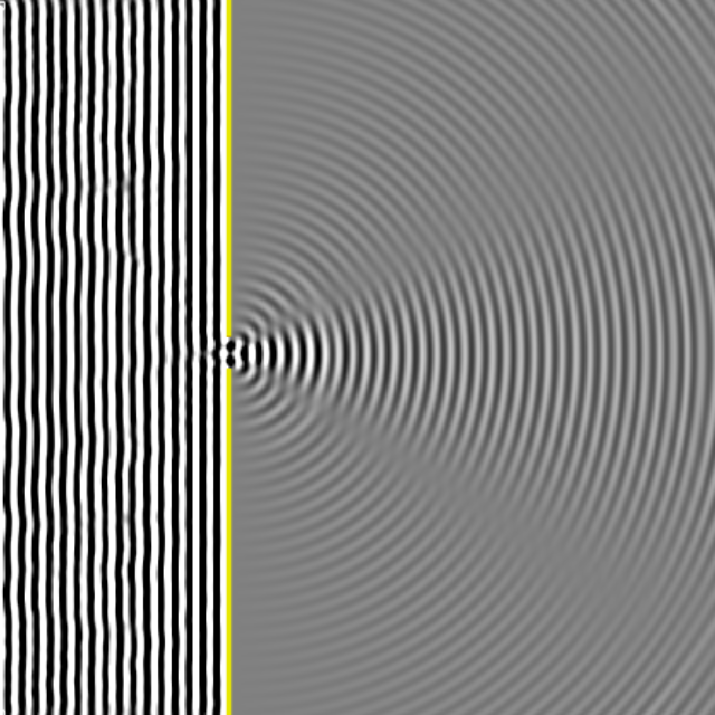
\includegraphics[width=9cm]{01_signaux_harmoniques_propagation/diffraction.png}};

\begin{scope}[x={(image.north east)}, y={(image.south west)}, shift={(0.319,0.493)}]
        \draw          (0,0)          -- (-31.827:0.65);
        \draw [dashed] (-31.827:0.65) -- (-31.827:0.75);
        
        \draw          (0,0)          --  (31.827:0.65);
        \draw [dashed] (31.827:0.65)  --  (31.827:0.75);
        
        \draw [dashed] (0.2,0) -- (0,0);
        \draw [->] (0.2,0) arc (0:-31.827:0.2) node [midway, right] {$\theta$};
        
        \draw [dashed] (0,0.023)    -- +(0.3,0);
        \draw [dashed] (0,-0.023)   -- +(0.3,0);
        \draw [<->] (0.3,-0.023) -- node [right] {$a$} (0.3,0.023);
\end{scope}
\end{tikzpicture}
\end{center}
\end{figure}
\end{propriete}

\begin{remarque}
Ce phénomène n'est donc pas perceptible pour de trop grandes valeurs de $a$, c'est à dire telles que $a \gg \lambda$.
\end{remarque}